\chapter{Cristales semiconductores} \label{Ch:09}

Como ya se describió en capítulos anteriores, un semiconductor no es sino un aislantes (a $T=0$K) pero con un gap de energía suficientemente pequeño ($\varepsilon_g <1$ eV) como para que, digamos a temperatura ambiente, una proporción apreciable de la banda de valencia (B.V.) pasan a ocupar la banda de conducción (B.C.). Estos electrones térmicamente excitados y los huecos que dejan de la B.V. pueden transportar corriente eléctrica (figura \ref{Fig:09-01}).


\begin{figure}[h!] \centering
	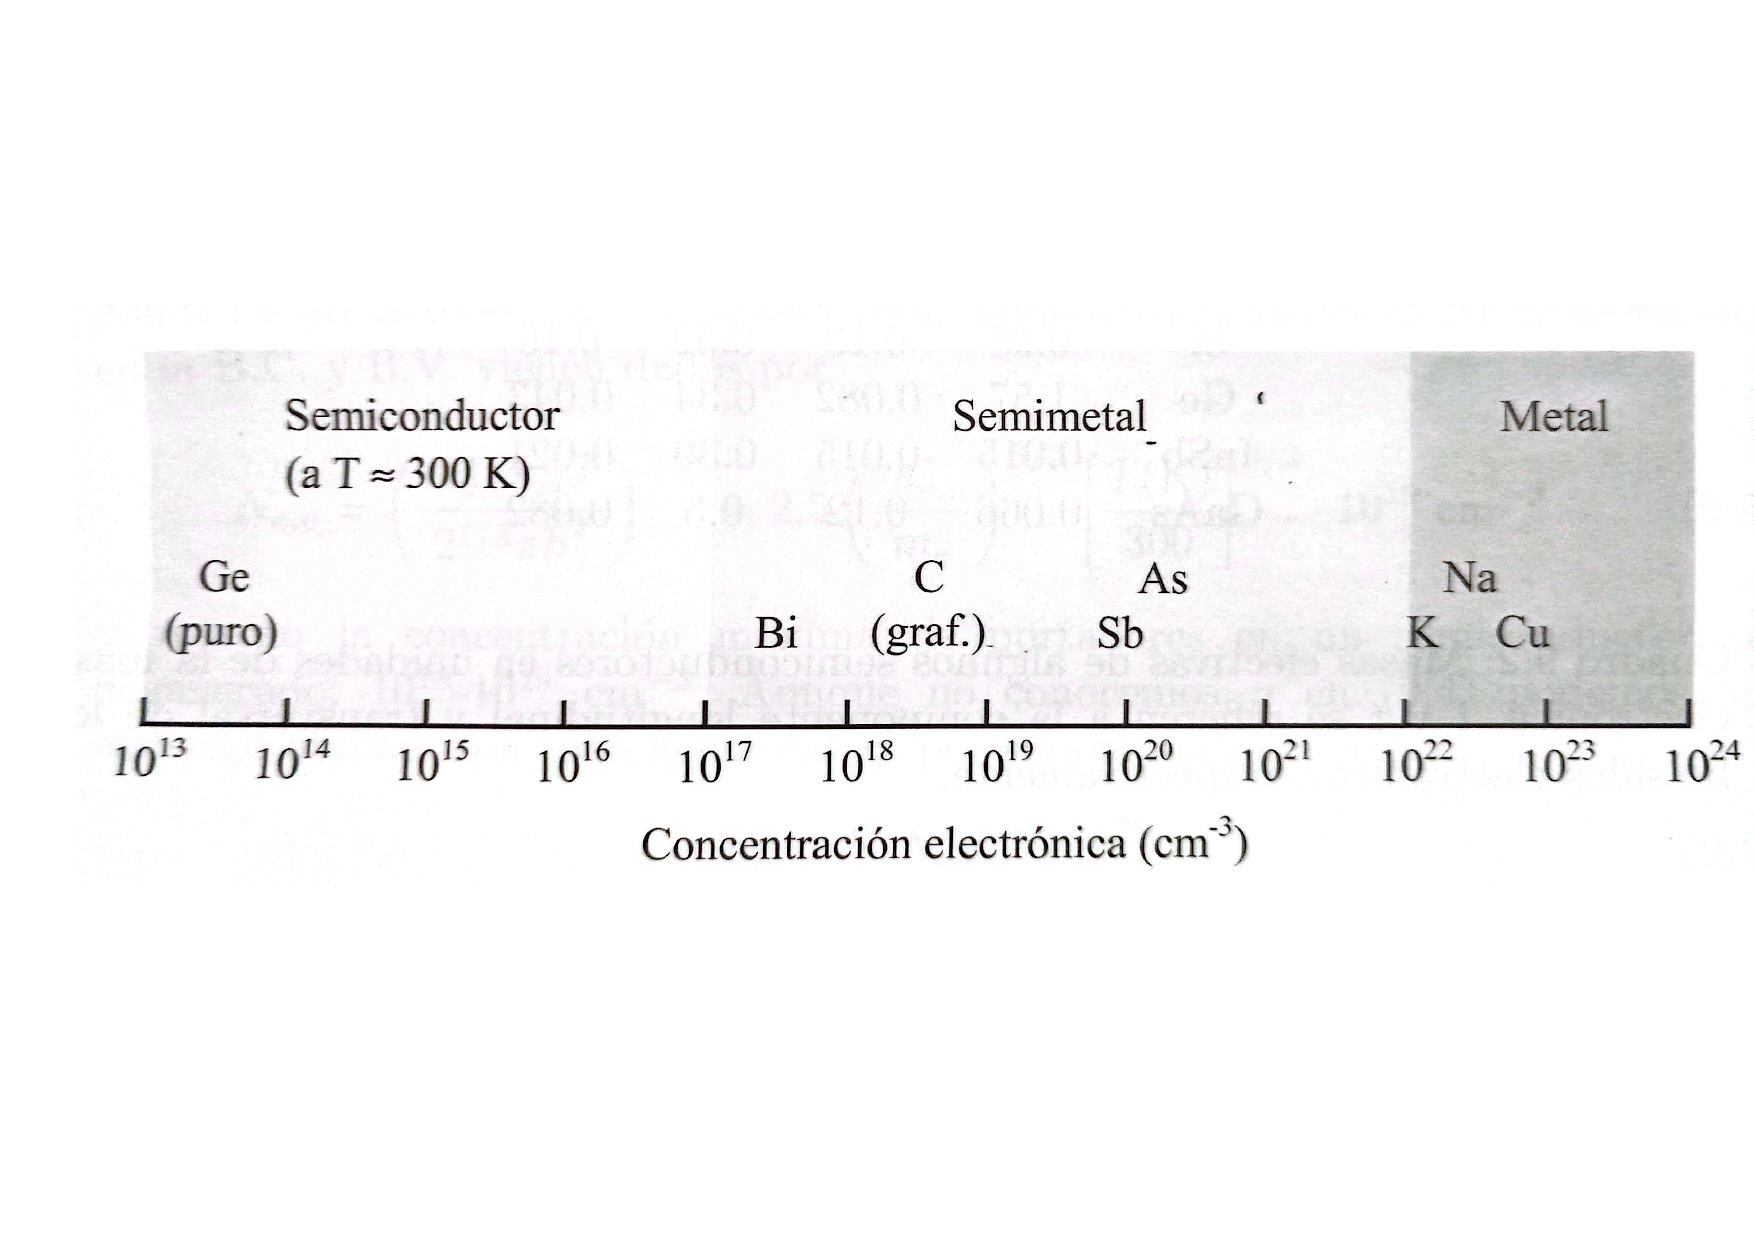
\includegraphics[scale=0.52]{Cuerpo/Ch_09/Fotos libro 1.pdf}
	\caption{Concentración de portadores para algunos metales, semimetales y semiconductores.}
	\label{Fig:09-01}
\end{figure}

Una propiedad especial de los semiconductores, que no se encuentra en metales, es que su conductividad eléctrica se puede alterar en muchos órdenes de manitud añadiendo pequeñas cantidades de otros elementos, que se denominan genéricamente \textit{impurezas}. Éstas determinan el carácter electrón o hueco de la conducción. Toda la electrónica de estado sólido (transistores, conmutadores diodos, células fotovoltaicas, etc.) descansa en esta propiedad conocida como \textit{dopado}.

Los semiconductores son generalmente cristales de enlace covalente. Los más comunes son los del grupo IV y los compuestos de los grupos III-V. El gap de energía $\varepsilon_g$ de algunos materiales se muestra en la tabla \ref{Tab:09-01}. Obsérvese la suave dependencia de $\varepsilon_g$ con la temperatura, debida en parte a la variación del espacio atómico (dilatación).

\begin{table}[h!] \centering
\begin{tabular}{ccc}
	Cristal & $\varepsilon_g$ (0 K) & $\varepsilon_g$ (300 K) \\ \hline
	Si & 1.17 & 1.12 \\
	Ge & 0.75 & 0.6 \\
	InSb & 0.23 & 0.17 \\ 
	GaAs & 1.52 & 1.43 \\
	Te & 0.33 & - \\ 
	SiC & 43.0 & - \\
	C (dia) & 5.5 & 5.5
\end{tabular}
\caption{Gap de energía para algunos materiales semiconductores.}
\label{Tab:09-01}
\end{table}
Otro parámetro fundamental es la masa efectiva, algunos de cuyos valores numéricos se muestran en la tabla \ref{Tab:09-02}. Hay dos masas de huecos porque en estos semiconductores hay dos bandas de valencia degeneradas (los máximos coinciden), pero que tienen distinta curvatura y, por tanto, distintas masas efectivas:

\begin{table}[h!] \centering
	\begin{tabular}{ccccc}
		Cristal & $m_l$ & $m_t$ & $m_h$ & $m_h'$ \\ \hline
		Si & 0.98 & 0.19 & 0.52 & 0.16 \\
		Ge & 1.57 & 0.082 & 0.34 & 0.043 \\
		InSb & 0.015 & 0.015 & 0.39 & 0.021 \\
		GaAs & 0.066 & 0.12 & 0.5 & 0.082
	\end{tabular}
	\caption{Masas efectivas de algunos semicondctores en unidades de la asa electrónica. $l$ y $t$ se refieren a la componente longitudinal y transversal de los bolsillos electrónicos, respectivamente.}
	\label{Tab:09-02}
\end{table}

\section{Concetración de portadores en equilibrio térmico}

Una propiedad fundamental de un semiconductor a temperatura $T$ es la concetración electrónca $n$ en la B.C. y la de los huecos $p$ en la B.V. Si denotamos por $D_c(\varepsilon)$ y $D_v(\varepsilon)$ las correspondientes densidades de estados por unidad de volumen, tendremos:

\begin{equation}
\begin{split}
	n \ = \ & \int_{\varepsilon_c}^{\infty} D_c (\varepsilon) f_{FD} (\varepsilon,T) \D \varepsilon \\
	p \ = \ & \int_{-\infty}^{\varepsilon_v} D_v (\varepsilon) [1-f_{FD}(\varepsilon,T)]\D \varepsilon
\end{split}\label{Ec:09-01-01}
\end{equation}
En la aproximación parabólica ($m^* = \cte$) la densidad de estados es una generalización directa de la obtenida para electrones libres. En concreto se encuentra

\begin{equation}
	D_{c,v} (\varepsilon) = \sqrt{2\abs{\varepsilon-\varepsilon_{c,v}}} \frac{m_{c,v}^{*3/2}}{\hbar^3 \pi^2}
\end{equation}
siendo $m_{c,v}^*=(m_1^*m_2^*m_3^*)^{1/3}$ la masa efectiva media geométrica de los valores principales del tensor de masa efecgiva de la B.C. y B.V. respectivamente. En todo lo que sigue adoptareos como válidas las condiciones:

\begin{equation}
\begin{split}
\varepsilon_c  - \mu & \gg k_B T \\
\mu - \varepsilon_v & \gg k_B T
\end{split} \label{Ec:09-01-03}
\end{equation}
en cuyo caso se dice no degenerado y se puede aplicar la estadística de Maxwell-Boltzmann en vez de la de Fermi-Dirac. En estas econdiciones las ecuaciones (\ref{Ec:09-01-01}) se reducen a:

\begin{equation}
	\begin{split}
		n = & N_c (T) e^{- \frac{\varepsilon_c - \mu}{k_B T}} \\
		n = & N_v (T) e^{- \frac{\mu-\varepsilon_v}{k_B T}} 
	\end{split} \label{Ec:09-01-04}
\end{equation}
donde los prefactores $N_c$ y $N_v$, a veces denominadas desidades efectivas de estados de la B.C. y B.V. vienen dados por

\begin{equation}
	N_{c,v}= \parentesis{\frac{m_{c,v}^* k_B T}{2^{1/3} \pi \hbar^2}}^{3/2} = 2.5 \parentesis{\frac{m_{c,v}^*}{m_e}}^{3/2} \ccorchetes{\frac{T(\text{K})}{300}}^{3/2} \cdot \unit{10^{19} \cm^{-3}} \label{Ec:09-01-05}
\end{equation}
y marcan la concetración máxima de portadores en un semiconductor no degenerado: $\unit{10^{18}-10^{19} \cm^{-3}}$. Aunque no concemos $\mu$ en (\ref{Ec:09-01-04}) podemos sin embargo obtener con toda generalidad, por simple multiplicación 

\begin{equation} 
	n p = N_c N_v e^{-\varepsilon_g/k_BT}\label{Ec:09-01-06}
\end{equation}
que se conoce como \textit{ley de acción de masas}, y donde ya no interviene $\mu$. En el caso de un semiconductor \textit{intrínseco}, que es aquél donde las impurezas no tienen influencia relevante (por ejemplo porque su número es despreciable), deberá ocurrir que $n=p=n_i$, lo que permite obtener de (\ref{Ec:09-01-04}) y (\ref{Ec:09-01-06})

\begin{equation}
	n_i = \sqrt{N_cN_v}e^{-\varepsilon_g/2k_BT} \label{Ec:09-01-07}
\end{equation}
Por ejemplo, $n_i(300\unit{\K})\approx\unit{10^{10}\cm^{-3}}$ en el Si. Asimismo, se obtiene

\begin{equation}
	\mu = \varepsilon_v + \frac{1}{2} \varepsilon_g + \frac{3}{4} k_B T \ln \parentesis{\frac{m_v^+}{m_c^+}} \label{Ec:09-01-08}
\end{equation}
de modo que $\mu$ está situado aproximadamente en la mitad del gap. La figura \ref{Fig:09-02} ilustra algunas de las relaciones encontradas.
\begin{figure}[h!] \centering
	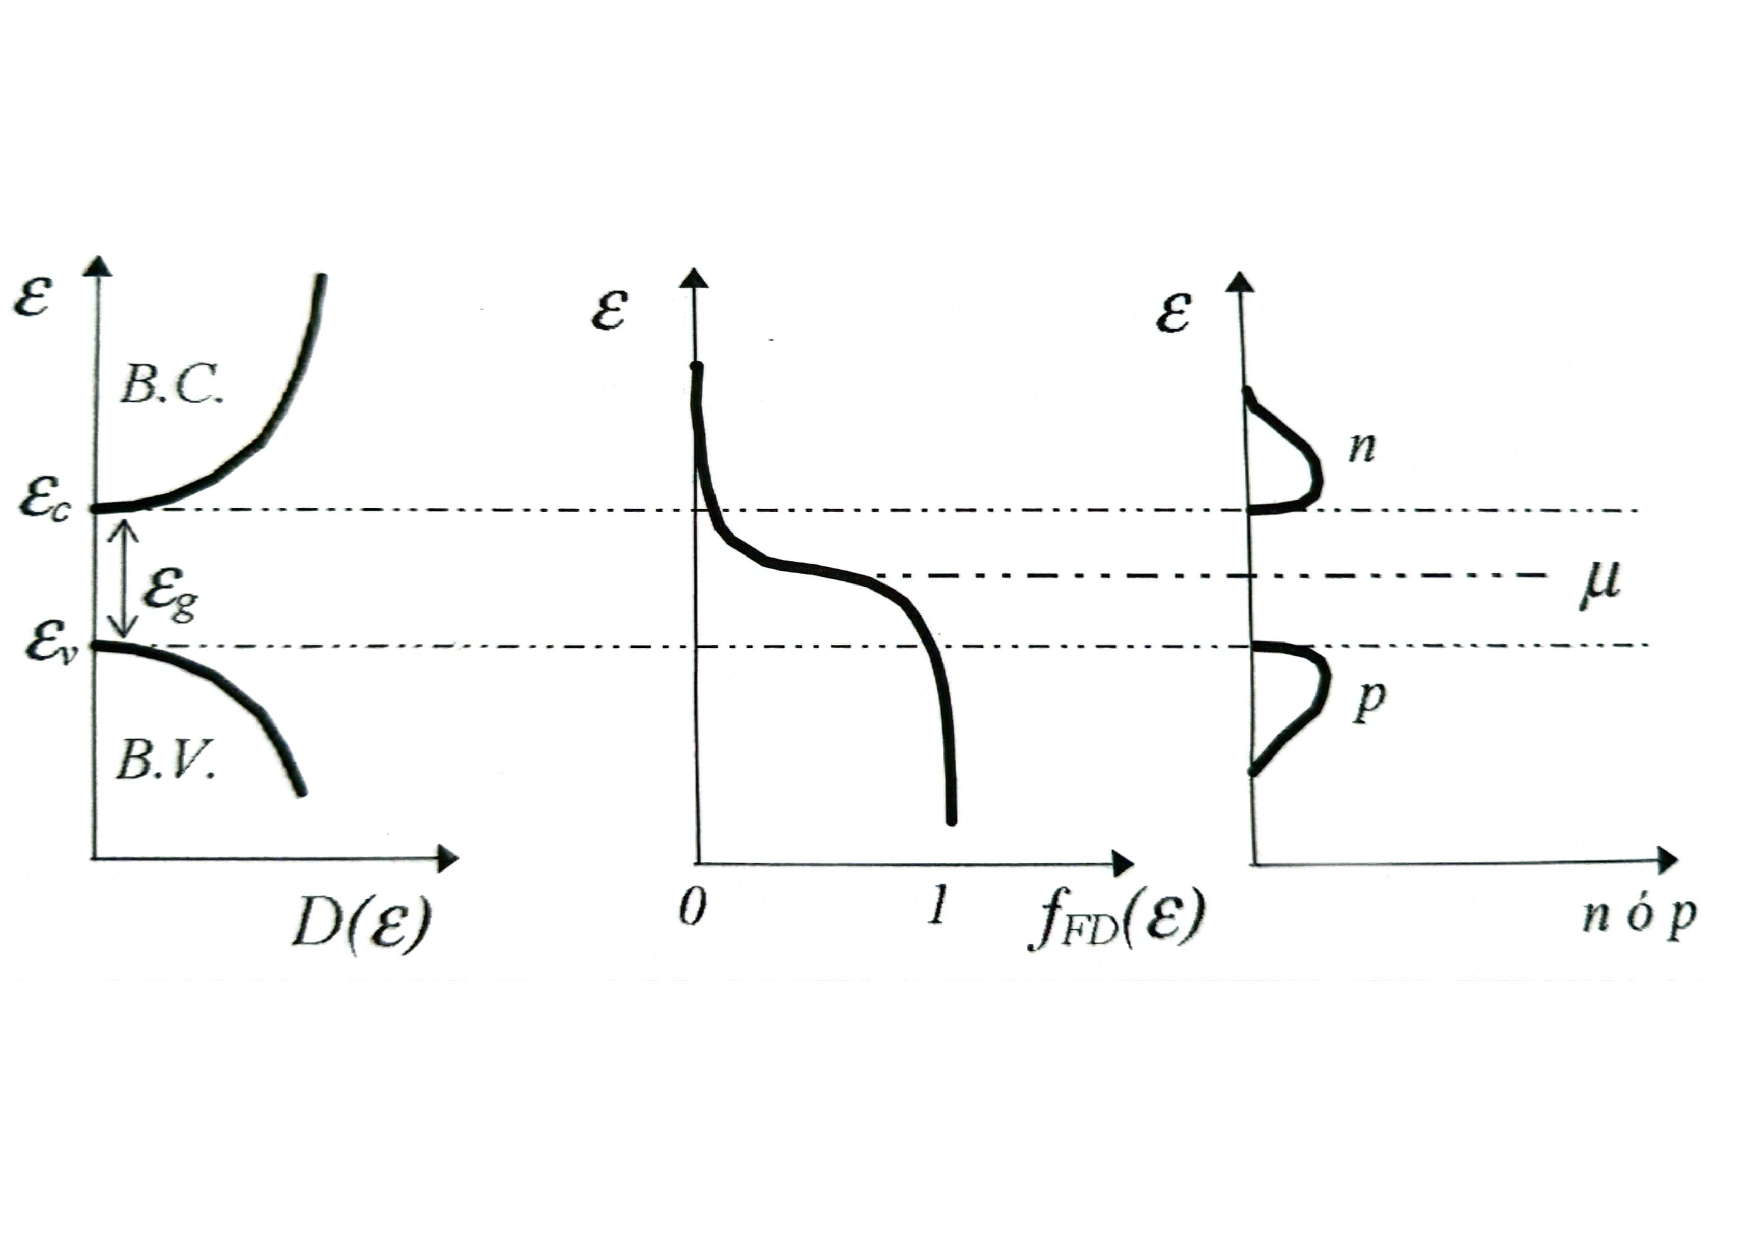
\includegraphics[scale=0.4]{Cuerpo/Ch_09/Fotos libro 2.pdf}
	\caption{Densidad de estados, ocupación de estados, y concetración de huecos y electrones para un semiconductor intrínseco.}
	\label{Fig:09-02}
\end{figure}

\section{Semiconductores dopados}

La manera de incrementar y controlar los portadores de carga en un semiconductor es dopándolo, esto es, añadiendo sustitucionalmente ciertas impurezas eléctricamente activas. Las impuras que aportan electrones (huecos) son normalmente elementos del grupo V (III) que se llaman dadoras (aceptores) y entonces el semiconductor se dice de tipo $n$ (tipo $p$). Supongamos por concretar un semiconductor del grupo IV, como  el Ge, dopado con impurezas dadoras repartidas aleatoriamente en el cristal. Cada una se puede considerar un centro de carga +$e$ al que está ligado un electrón, ya que los otros cuatro están ya ocupados formando los cuatros enlaces covalentes de la estructura del diamante. La energía necesaria para ionizar la impureza, pasando entonces el electrón del estado ligado localizado al estado libre deslocalizado (es decir, a la B.C.), es relativamente baja. Esto se debe a que el electrón en exceso ve un potencial periódico además de un centro de carga atractor $+e$, lo que significaba pasar de $m$ a $m^*$. Pero además, el electrón está en un medio dieléctrico (polarizable) que es el propio semiconductor, lo que implica pasar de $e^2$ a $e^2/\kappa$ siendo $\kappa$ la permitividad eléctrica relativa del medio, por ejemplo $\kappa(\ce{Ge})=15.8$, $\kappa(\ce{Si})=11.7$. Cuantitativamente se procede utilizando las fórmulas del átomo de hidrógeno. Así el radio de la primera órbita de Bohr $a_0=\hbar^2 / 2me^2=0.53 \ \unit{\angstrom}$ pasa a ser
 
\begin{equation}
	a_d = \frac{m}{m^*} \kappa a_0
\end{equation}
y la energía de ionización $\varepsilon_0=me^4/2\hbar^2=13.6 \ \unit{\eV}$ queda en

\begin{equation}
	\varepsilon_d = \frac{m^*}{m} \frac{1}{\kappa^2} \varepsilon_0
\end{equation}
Para valores típicos de $m^*$ y $\kappa$, $a_d$ puede ser $10^2 \ \unit{\angstrom}$ o más, y $\varepsilon_d$ puede quedar en $0.01-0.1 \ \unit{\eV}$. Argumentos similares se pueden desarrollar para las impurezas aceptoras, que se ionizan fácilmente (energía de ionización $\varepsilon_a$) captando un electrón de la B.V. Este electrón que ahora está localizado deja un hueco ``libre'' en la B.V. que contribuye a la conducción. Las impurezas dadoras generan un nuevo nivel  energético ($\varepsilon_D$) situado una energía $\varepsilon_d$ por debajo de la banda de conducción, y las aceptoras generan otro nivel ($\varepsilon_A$) situado una energía $\varepsilon_a$ por encima de la banda de valencia (ver figura \ref{Fig:09-03}).

\begin{figure}[h!] \centering
	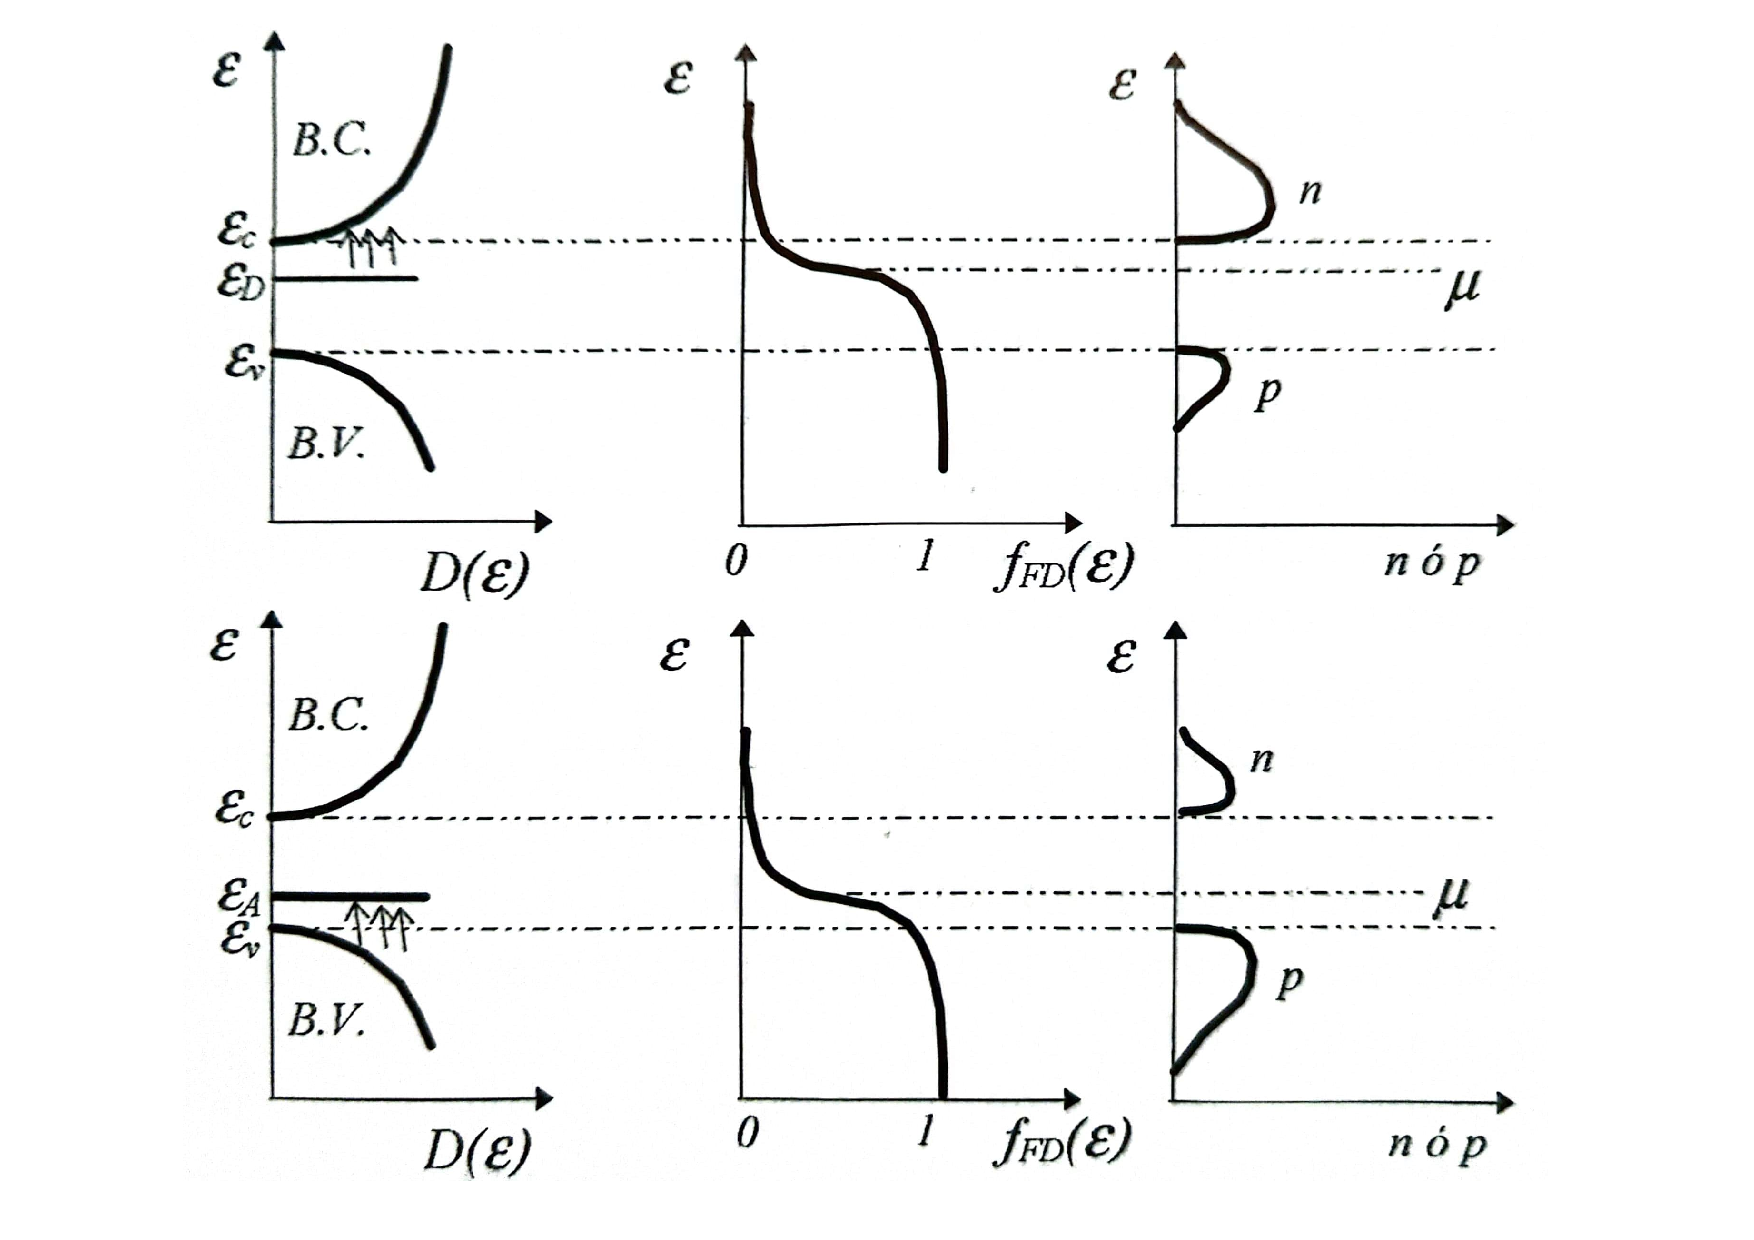
\includegraphics[scale=0.35]{Cuerpo/Ch_09/Fotos libro 3.pdf}
	\caption{Densidad de estados, ocupación de estados, y concentración de huecos y electrones para semiconductores con impurezas dadoras (arriba), o aceptoras (abajo).}
	\label{Fig:09-03}
\end{figure}

La información fundamental respecto a los niveles de asociados a las impurezas es su grado de ocupación a una temperatura determinada. En el caso de impurezas aceptoras esta coincidirá con la impurezas ionizadas (que han captado un electrón de la banda de valencia). Utilizando la mecánica estadística es fácil comprobar que a una temperatura determinada la concetración de impurezas aceptoras ionizadas viene dada por

\begin{equation}
	N_A^- = \frac{N_A}{1+2e^{(\varepsilon_A-\mu)/k_BT}} \label{Ec:09-02-03}
\end{equation}
donde $N_A$ es la concetración total de impurezas aceptoras. Nótese la similitud de esta expresión con la distribución de Fermi-Dirac (la diferencia es debida a que la repulsión entre $e^-$ localizados hace muy improbable la ocupación de la impureza con dos electrones simultáneamente). En el caso de impurezas dadoras, la proporción de impurezas ionizadas (que han donado un $e^-$ a la banda de conducción) coincidirá con el grado de \textit{desocupación} de los niveles asociados. De manera análoga, se encuentra que la concetración de dichas impurezas ionizadas a una temperatura dada viene dada por
 
\begin{equation}
	N_D^+ =  \frac{N_D}{1+2e^{(\mu-\varepsilon_D)/k_BT}} \label{Ec:09-02-04}
\end{equation}
donde ahora $N_D$ es la concentración total de impurezas dadoras.

\section{Concentración de portadores en Semiconductores dopados}

La cercanía de los niveles dadores y aceptoras a las bandas hace esperar en un semiconductor dopado, por ejemplo tipo $n$, sesa mucho más probable la promoción de electrones a la B.C. desde los niveles dadores que desde la B.V. Dicho de otro modo, la concentración de portadores estará controlada por las impurzas; el semiconductor se dice entonces en \textit{régimen de ionización}. Una vez todas las impurezas dadores están ionizadas (esto ocurre a partir de la llamada \textit{temperatura de saturación}, $T_s \leq 100 \ \unit{K}$) se entra en el \textit{régimen de saturación}, en que $n\approx N_D$ y por tanto independientes de la temperatura (numéricamente $10^{14}<N_D<10^{18} \unit{cm^{-3}}$). Los electrones se dicen en este caso portadores mayoritarios y correspondientes, por la ley de acción de masas, los huecos son minoritarios. Al aumentar la temperatura deberá ocurrir que el número de electrones procedentes de la B.V. supere el debido a las impurezas, de modo que $n\gg N_D$ entrándose entones en el \textit{régimen intrínseco}, en que la presencia de impurezas resulte irrelevante y $n\approx n_i$. La temperatura a partir de la cual se entra en este régimen se conoce como \textit{temperatura intrínseca}, $T_i$. Argumentos similares, aunque complementarios, se pueden aducir para semiconductores tipo $p$. La figura \ref{Fig:09-03}, ilustra el efecto de las impurezas.

El estudio Cuantitativamente parte de las expresiones (\ref{Ec:09-01-01}) para la concentración de portadore en las bandas que, por la generalidad de su obtención, siguen siendo válidas en presencia de impurezas. No obstante, desconocemos el potencial químico, pues la expresión (\ref{Ec:09-01-08}) vista no es ahora válida, ya que al haber aporte extra de electrones y/o huecosya no se verifica la condición $n=p$. La generalización de esta condición en presencia de impurezas es 

\begin{equation}
	n+N_A^- = p + N_D^+ \label{Ec:09-03-01}
\end{equation}
llamado condición de \textit{electroneutralidad}. La utilización consiste en sustituir (\ref{Ec:09-01-01}), (\ref{Ec:09-02-03}) y (\ref{Ec:09-02-04}) en (\ref{Ec:09-03-01}) con objeto de delimitar $\mu$ y llevarlo luego a (\ref{Ec:09-01-01}) para conocer la conetración de portadores a cualquier temperatura. Cualitativamente la evolución de $n$ en función de la temperatura para un semiconductor tipo $n$ es el que ilustra la figura \ref{Fig:09-04}.

\begin{figure}[h!] \centering
	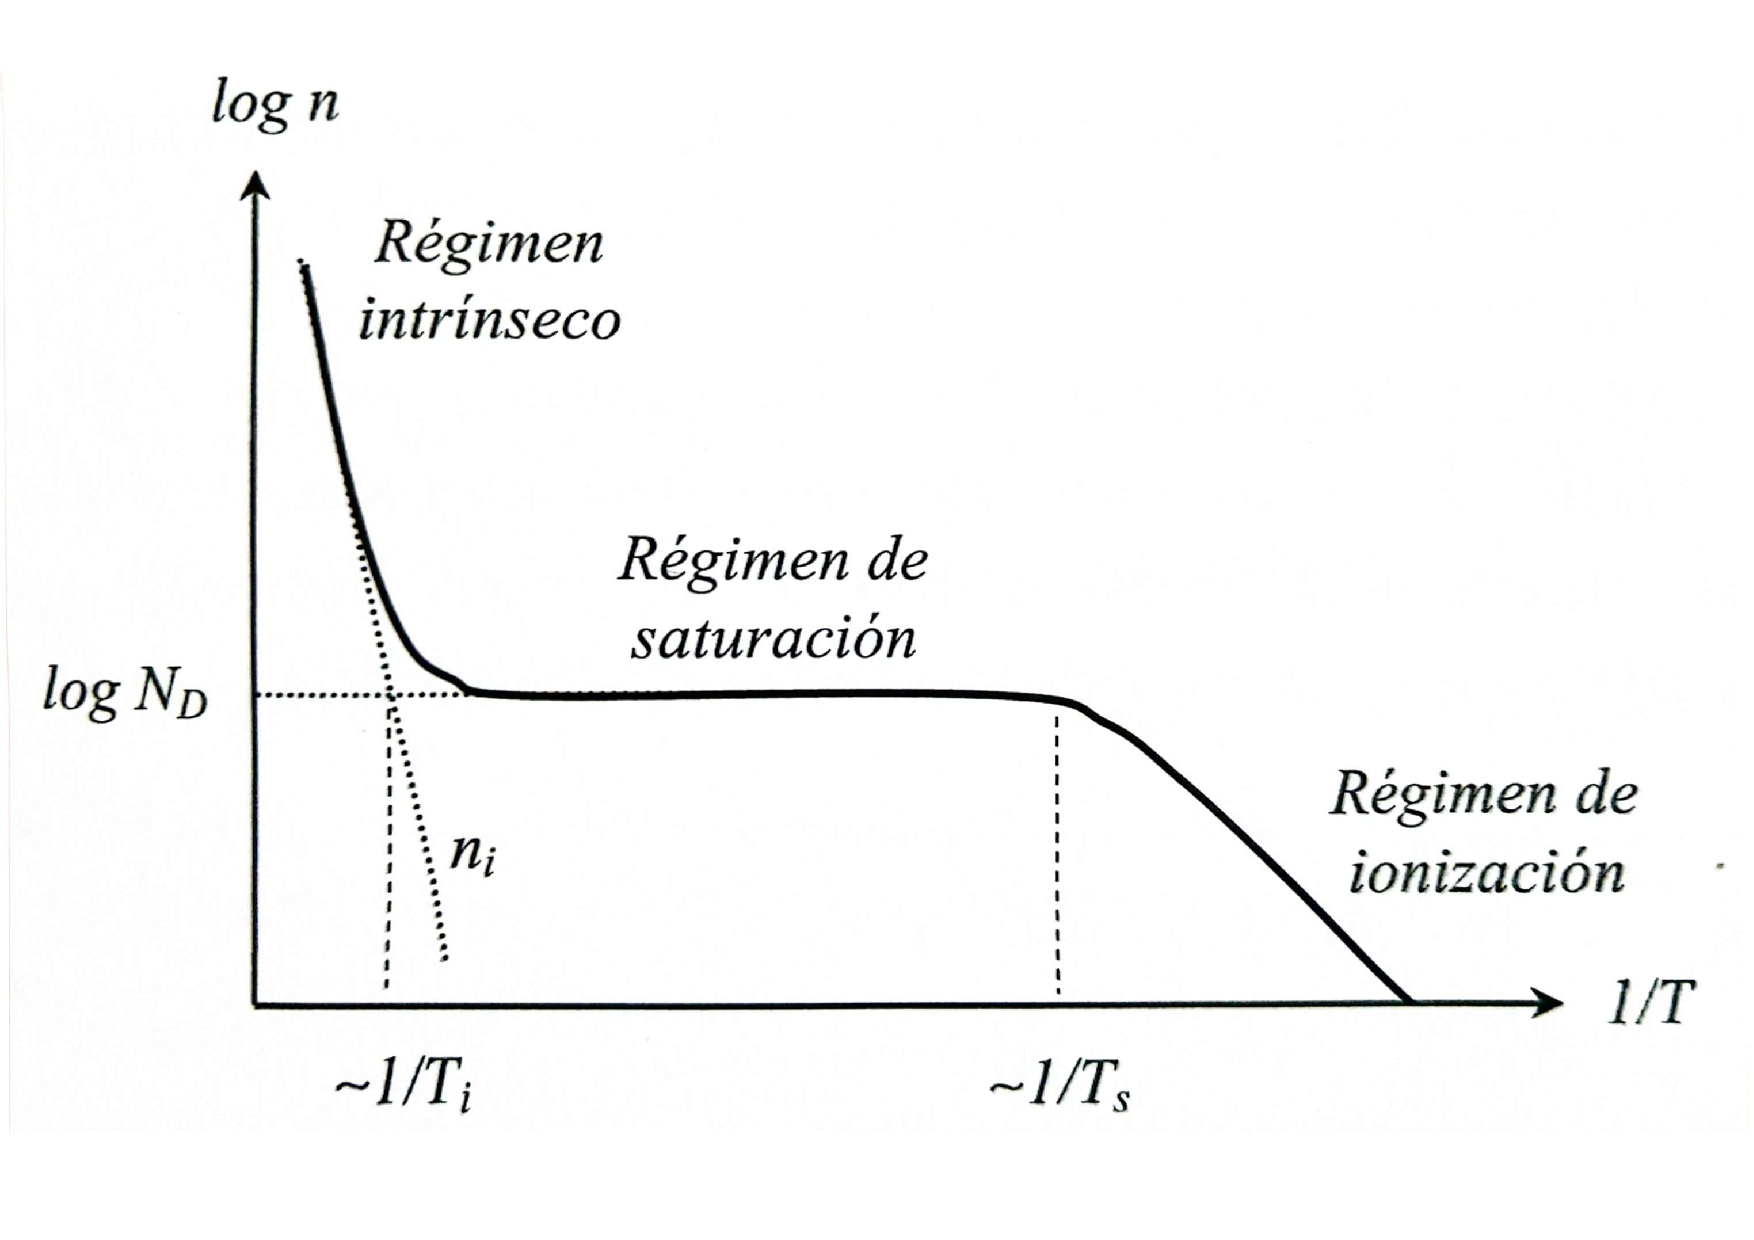
\includegraphics[scale=0.35]{Cuerpo/Ch_09/Fotos libro 4.pdf}
	\caption{Dependencia con la temperatura de la concentración de portadores en un semiconductor dopado con impurezas dadoras.}
	\label{Fig:09-04}
\end{figure}

\section{Conductividad y movilidad}

Consideraremos sólo semiconductores no degradados, es decir, aquéllos para los que la aproximación de Boltzmann (\ref{Ec:09-01-03}) es válida. Las contribuciones a la conductividad eléctrica debidas a electrones en la B.C. y a huecos en la B.V. se expresan por 

\begin{equation}
\begin{split}
	\sigma_n = & \frac{ne^2 \bar{\tau}_e}{m_c^*} \\	
	\sigma_p = & \frac{pe^2 \bar{\tau}_h}{m_v^*}
\end{split} \label{Ec:09-04-01}
\end{equation}
y la conductividad eléctrica total vendrá dada por $\sigma=\sigma_n + \sigma_p$. Los tiempos de relajación de la ecuación anterior (\ref{Ec:09-04-01}) son medias para todos los electrones en la B.C. y huecos en la B.V., pues todos ellos participan en la conducción: la aproximación de Boltzmann hace que la probabilidad de ocupación de un estado en B.V. o B.C. sesa muy pequeña por lo que un electrón y/o hueco tiene acceso a los niveles próximos, condición necesario para que se pueda ``acelerar''. Las ecuaciones (\ref{Ec:09-04-01}) pueden expresarse en función de las correspondientes \textit{movilidades} $\mu_n$ y $\mu_p$ según


\begin{equation}
	\begin{split}
		\sigma_n = en\mu_n \quad & \parentesis{\mu_n \equiv \frac{e^2 \bar{\tau}_e}{m_c^*}} \\	
		\sigma_p = ep\mu_p \quad & \parentesis{\mu_p \equiv \frac{e^2 \bar{\tau}_h}{m_v^*} }
	\end{split} \label{Ec:09-04-02}
\end{equation}
Los mecanismos básicos de dispersión de los portadores que afectan a la movilidad en semiconductores son: los fonones, como en metales, y las impurezas ionizadas a través de la dispersión de Rutherford (salvo a muy bajas temperaturas en que permanecen neutras). Sin entrar en detalles digamos que las dependencias respectivas con la temperatura son:

\begin{equation}
\begin{split}
\mu_{\text{fon}} & \propto T^{-3/2} \\
\mu_{\text{imp}} & \propto T^{3/2} \\
\end{split}
\end{equation}
Obsérvese que la movilidad por interacción con fonones disminuye al aumentar la temperatura por aumentar el número de éstos, pero sin embargo, la movilidad aumenta para la interacción con impurezas. La razón es que al aumentar la temperatura aumenta la velocidad de los portadores de modo que están menos tiempo en el radio de influencia de cada interacción. La figura \ref{Fig:09-05} muestra los dos regímenes comentados (el cambio de régimen depende de la concentración de impurezas, pero en general ocurre para $T<100\ \unit{K}$).

\begin{figure}[h!] \centering
	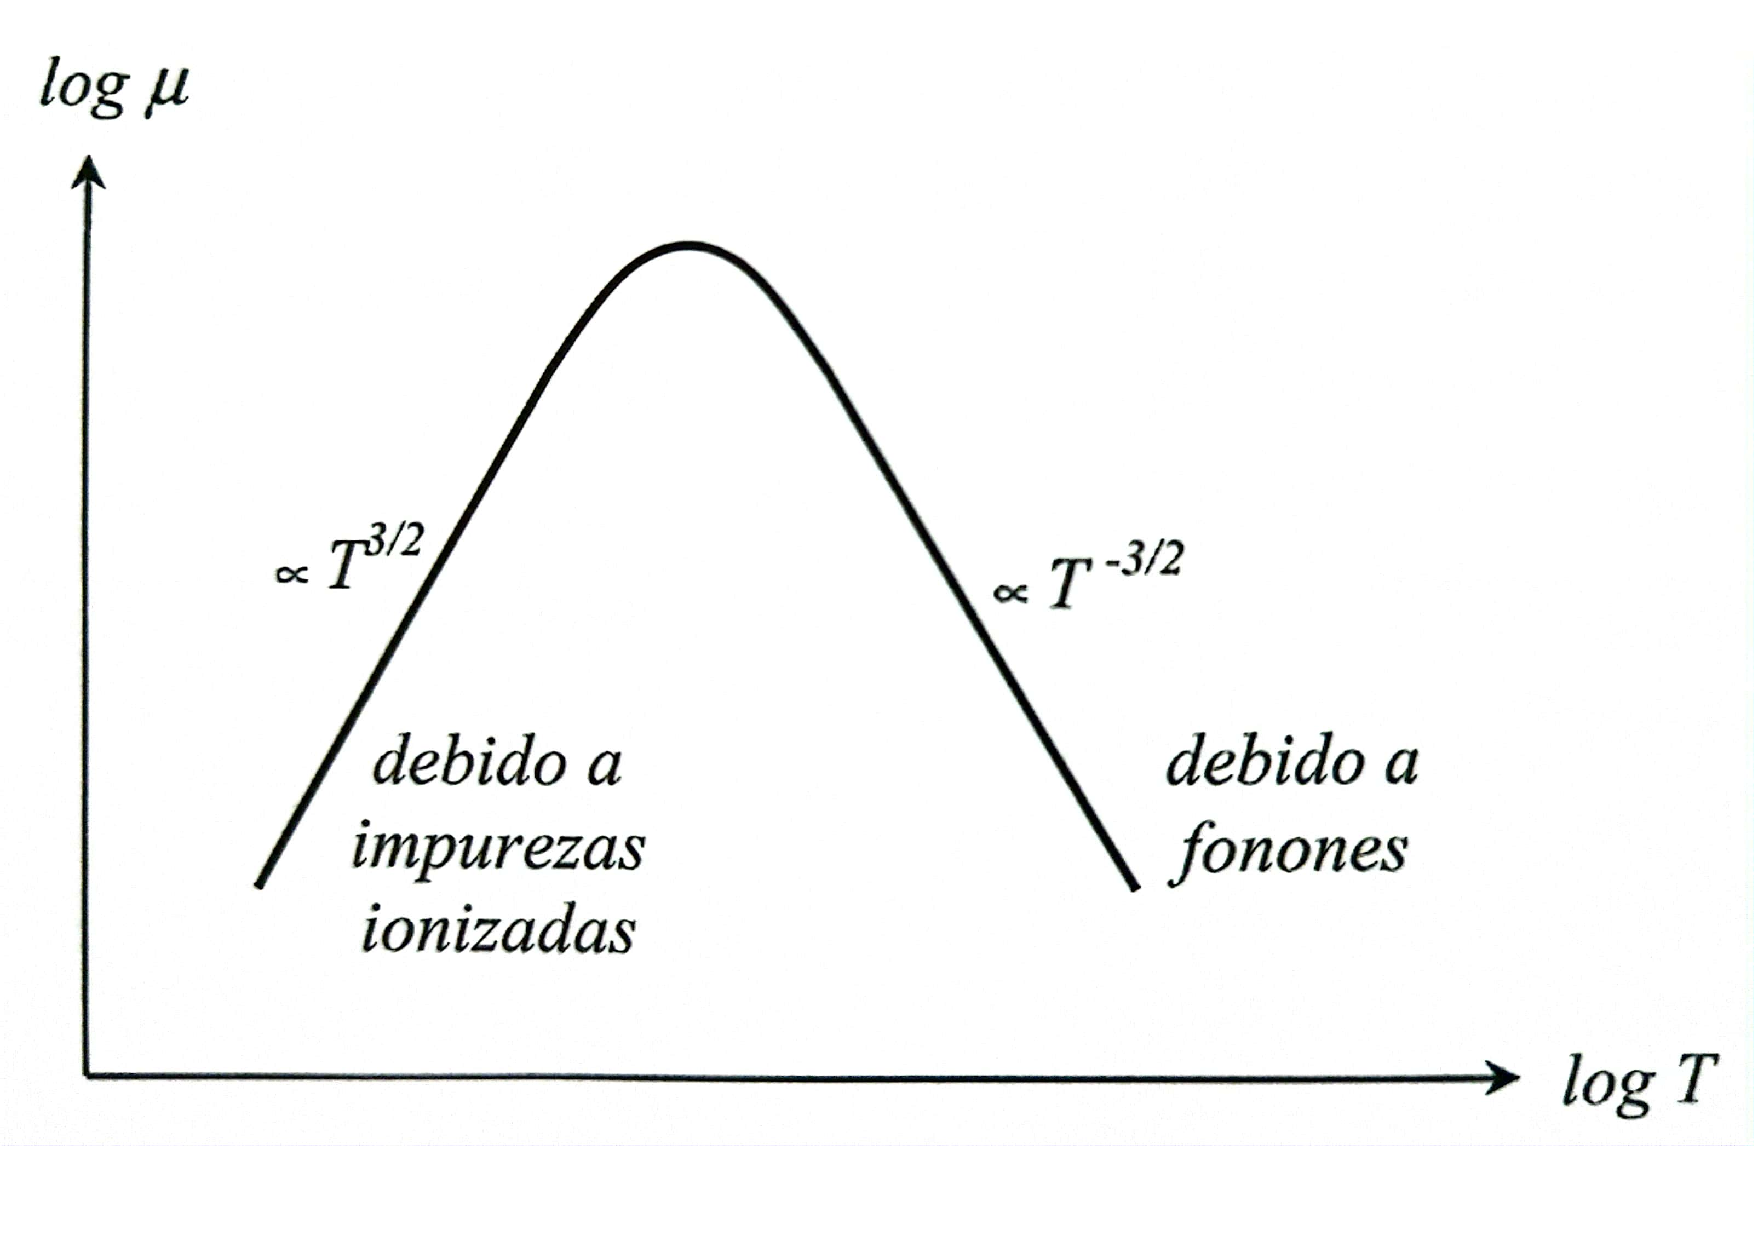
\includegraphics[scale=0.35]{Cuerpo/Ch_09/Fotos libro 5.pdf}
	\caption{Dependencia con la temperatura de la movilidad en un semiconductor con impurezas.}
	\label{Fig:09-05}
\end{figure}

Es interesante particularizar para un semiconductor intrínseco a \textit{alta temperatura}. A partir de (\ref{Ec:09-01-05}), (\ref{Ec:09-01-07}) y (\ref{Ec:09-04-02}) se encuentra para la conductividad eléctrica

\begin{equation}
	\sigma = en\mu_n + ep\mu_p \propto \parentesis{T^{3/2}e^{-\varepsilon_g/2k_BT}}T^{-3/2}  = e^{-\varepsilon_g/2k_BT}
\end{equation}
Este resultado proporciona un método sencillo para determinar el gap de energía de un semiconductor a partir de la conductividad en función de la temperatura.

\section{Semiconductores inhomogeneos: la unión p-n.}

Se estudia el comportamiento de una unión de un semiconductor tipo $p$ con otro tipo $n$, que es la base de buena parte de la microelectrónica. Cualitativamente, los electrones tienden a difundirse del lado $n$ donde son mayoritarios al $p$ donde son minoritarios, y viceversa para los huecos. Esta difusión origina un campo eléctrico en una región de dimensiones $d_n+d_p$ aldrededor de la superficie de separación que frena la difusión, llegándose así al equilibrio. Además, como los portadores son muy móviles, la concentración de los mismos debe ser muy baja allí donde el campo eléctrico es apreciable. Por tanto la ausencia de portadores libres en la región de campo hace que ésta aparezca cargada, tal como ilustra la figura \ref{Fig:09-06} justificando además el nombre de \textit{región de carga espacial} que recive. Típicamente $d_n+d_p\sim10^2 - 10^4 \unit{\angstrom}$ y el campo en la región de carga es $10^5 - 10^7$ V/m.


\begin{figure}[h!] \centering
	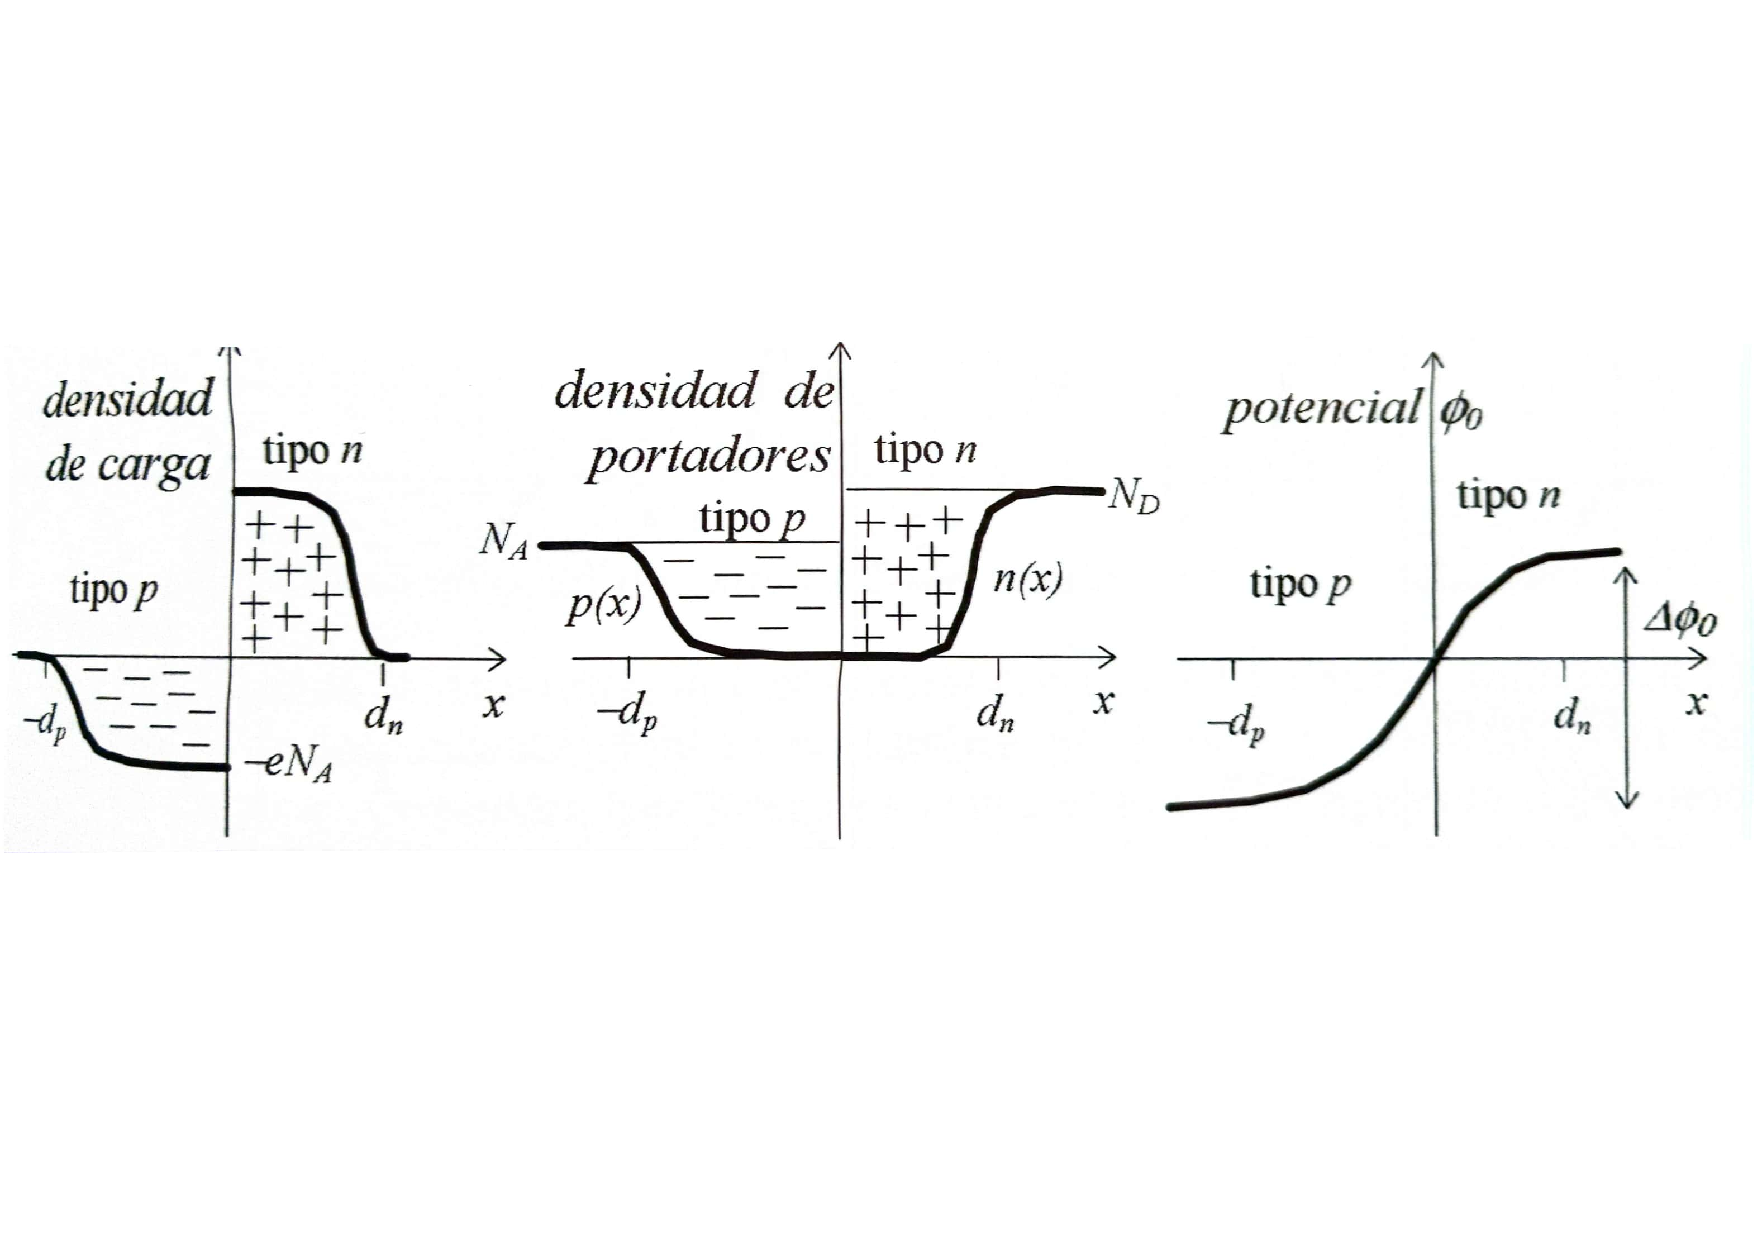
\includegraphics[scale=0.35]{Cuerpo/Ch_09/Fotos libro 6.pdf}
	\caption{Densidad de carga, densidad de protones, y potencial eléctrico en la región de caga especial de unión $p-n$.}
	\label{Fig:09-06}
\end{figure}

Vamos a considerar ahora qué ocurre se aplica un potencial externo $V$ (tomaremos $V>0$ si es más alto de lado $p$ que el lado $n$, ver \ref{Fig:09-07}). Puesto que muy cerca de la unión, en la capa de carga espacial, la concentración de portadores es casi nula, la resistencia eléctrica que ésta presenta será mucho mayor que en las regiones homogéneas. Esto implica que cuando se aplica un potencial $V$ a la unión de mayor caída se dará en la carga espacial. Queremos deducir aproximadamente la corriente eléctrica a través de la unión si $V\neq 0$. Para empezar, consideremos en detalle la corriente debida a huecos. Hay dos contribuciones:

\begin{itemize}
	\item La corriente de generación $j_h^{\text{gen}}$ del lado $n$ al $p$, que aparece por los huecos generados térmicamente del lado $n$ donde son minoritarios al lado $p$ donde son mayoritarios. Aunque la concentración es pequeño, la corriente a t ravés de la unión puedde ser alta ya que los huecos se ven lanzados por el campo eléctrico en la unión, y será poco sensible al valor de $V$ si $eV\gg \varepsilon_g$.
	\item La corriente de recombinación $j_h^{\text{rec}}$, del lado $p$ al lado $n$, debida a los huecos que, llegados a la unión del lado $p$, tengan energía suficiente para vencer el campo eléctrica en la misma. Esta corriente debida a hueos será:
	\begin{equation}
		j_h^{\text{rec}} \propto \exp \parentesis{-e\frac{\Delta \phi_0-V}{k_BT}} = j_h^{\text{rec}}|_{V=0} \exp \parentesis{\frac{eV}{k_BT}}
	\end{equation}
\end{itemize}
Se debe cumplir además que

\begin{equation}
	\parentesis{j_h^{\text{rec}}}_{V=0} = \parentesis{j_h^{\text{gen}}}_{V=0} \approx\parentesis{j_h^{\text{gen}}}_V
\end{equation}
por la pequeña dependencia de $J_h^{\text{rec}}$ al potencial externo; con esto

\begin{equation}
	j_h^{\text{rec}} = j_h^{\text{gen}} \exp \parentesis{\frac{eV}{k_BT}}
\end{equation}
de donde 

\begin{equation}
	j_h = j_h^{\text{rec}}  - j_h^{\text{gen}}  = j_h^{\text{gen}} \ccorchetes{\exp\parentesis{\frac{eV}{k_BT}}-1} 
\end{equation}
\begin{figure}[h!] \centering
	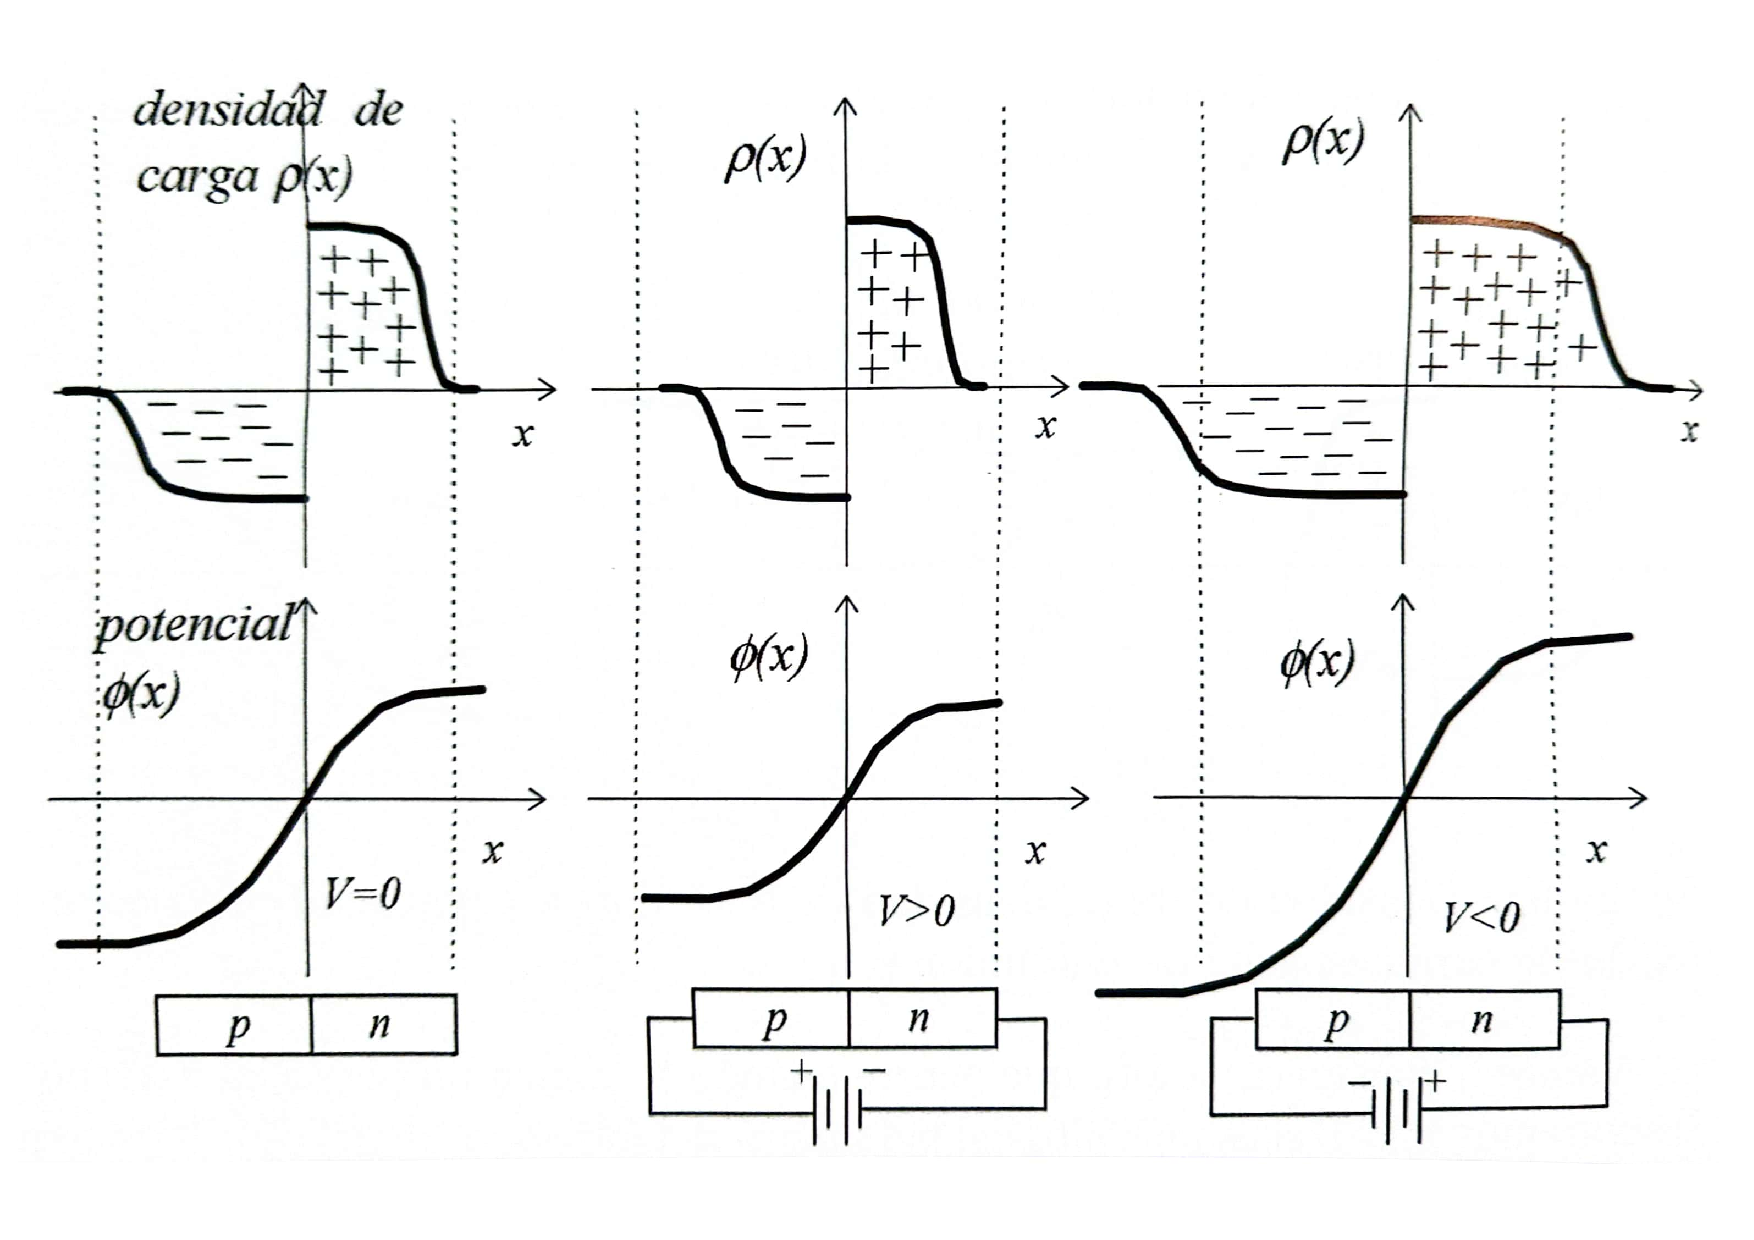
\includegraphics[scale=0.25]{Cuerpo/Ch_09/Fotos libro 7.pdf}
	\caption{Efecto de un potencial externo sobre la densidad de carga en la región de carga especial de unión $p-n$.}
	\label{Fig:09-07}
\end{figure}
Análogo análisis se aplica a los electrones, de forma que para la densidad de corriente eléctrica \textit{total} se tiene 
 
\begin{equation}
	j=\parentesis{j_h^{\text{rec}}-j_e^{\text{gen}}} \ccorchetes{\exp \parentesis{\frac{eV}{k_BT}}-1} \label{Ec:09-05-05}
\end{equation}
Se peude probar que el término $j_h^{\text{gen}}+j_e^{\text{gen}}$ varía con la temperatura según $\exp\parentesis{-\varepsilon_g/k_BT}$. La alta simetría de la unión respecto de la polarización en voltaje tal como resume la ecuación (\ref{Ec:09-05-05}) y se representa en la , constituye el principio \textit{rectificador} de la unión.

\begin{figure}[h!] \centering
	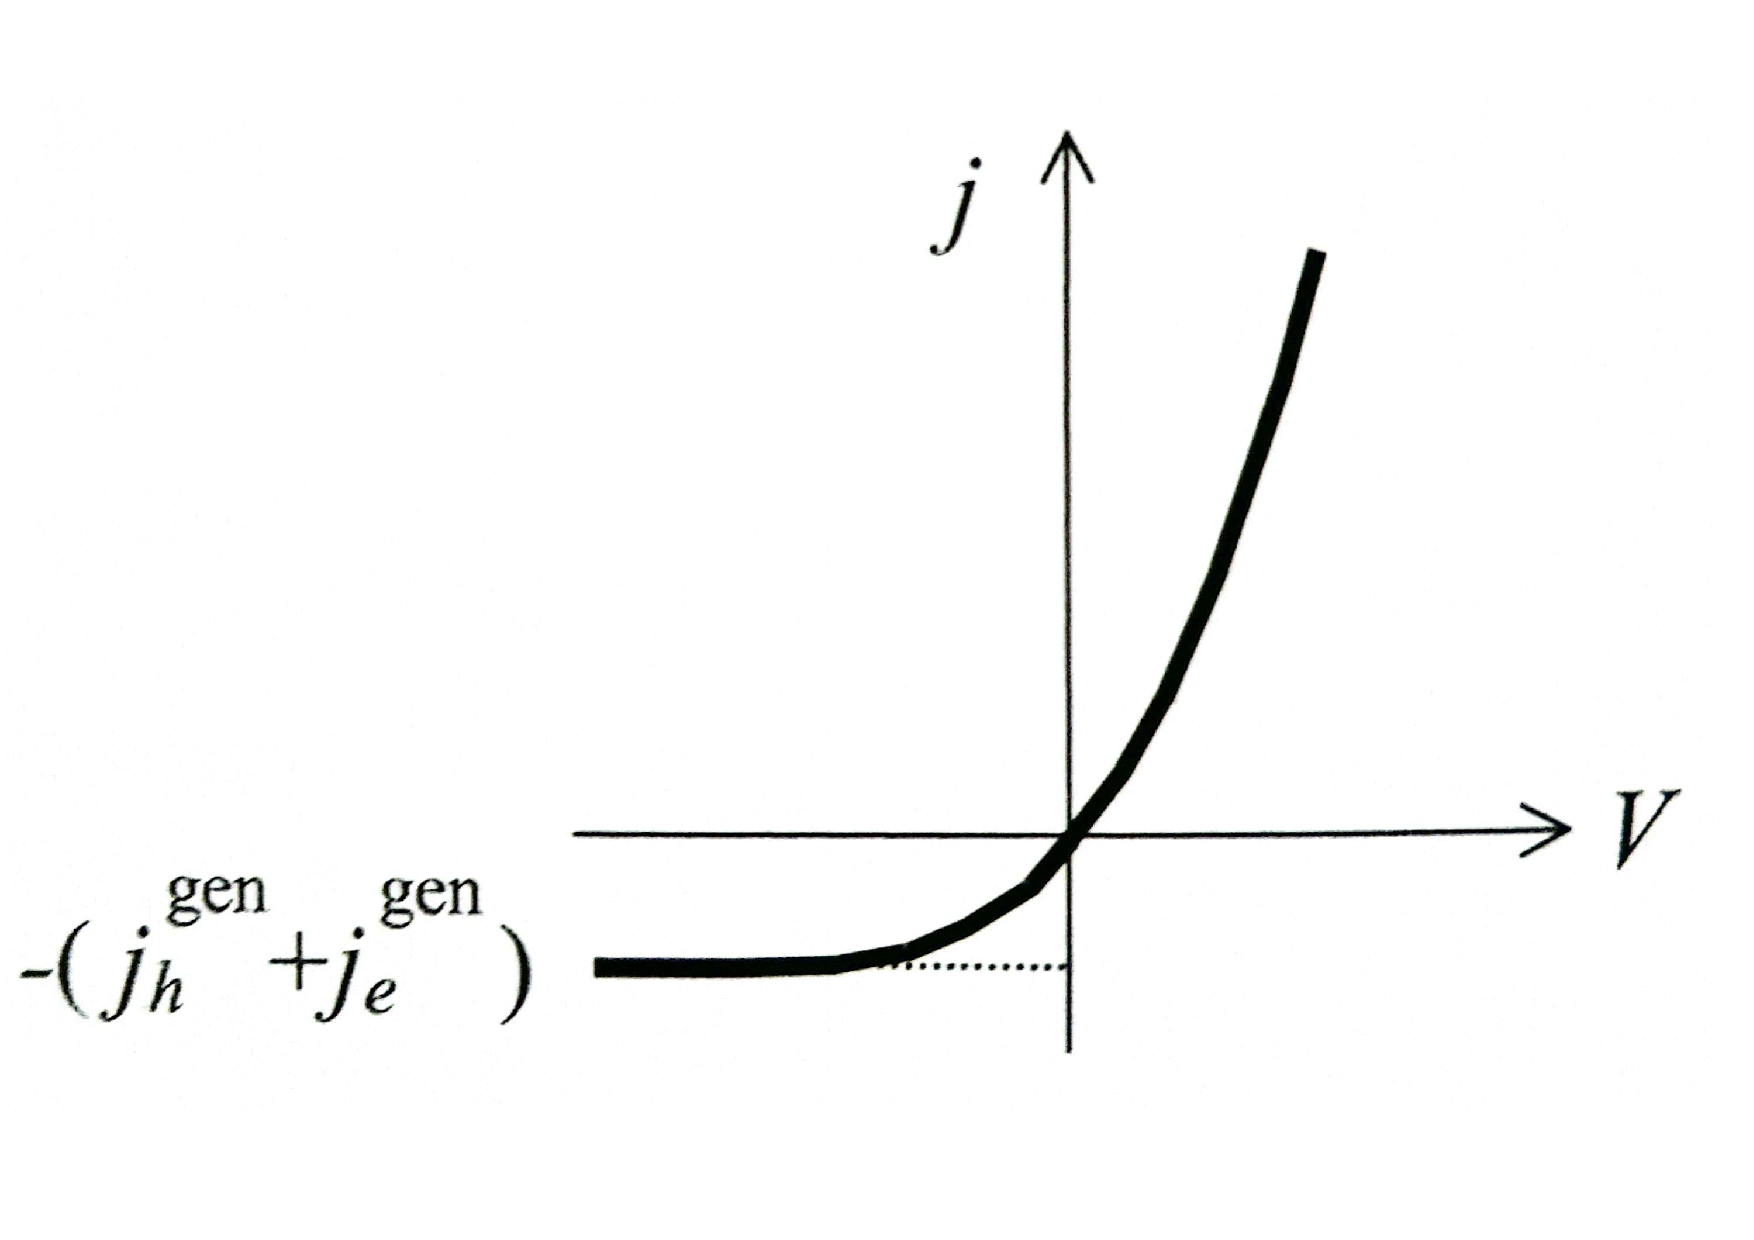
\includegraphics[scale=0.25]{Cuerpo/Ch_09/Fotos libro 8.pdf}
	\caption{Relación $j-V$ para la unión $p-n$.}
	\label{Fig:09-08}
\end{figure}